% Template for ICIP-2019 paper; to be used with:
%          spconf.sty  - ICASSP/ICIP LaTeX style file, and
%          IEEEbib.bst - IEEE bibliography style file.
% --------------------------------------------------------------------------
\documentclass{article}
\usepackage{spconf,amsmath,graphicx}
\usepackage[backend=biber, style=ieee]{biblatex}
\usepackage{float}
\addbibresource{reportRefs.bib}

% Example definitions.
% --------------------
\def\x{{\mathbf x}}
\def\L{{\cal L}}

% Title.
% ------
\title{House Price And Affordability In Regions Of Englanf And Wales}
%
% Single address.
% ---------------
% \name{Author(s) Name(s)\thanks{Thanks to XYZ agency for funding.}}

\name{Junsong Yang}
\address{4274056 \\
psyjy3@nottingham.ac.uk}

\begin{document}
%\ninept
%
\maketitle
%

\section{Introduction}
House price has changed dramatically over the past few years. Such changes are drawing attention as they are leading to housing affordability issues. For example, house price in London increased drastically these years, as a result, house price is becoming unaffordable
to most of the residents. Analysis of how the house price changed and to what extent the affordability is affected by those changes is provided.

This paper is intended to explore this issue based on data about house prices and affordability measurements. 
In general, there are four sections, Initial Question, Data Processing, Information Visualisation and Evaluation.
In the Initial Questions section, issues related to house prices will be discussed therefore research questions will be proposed. As for Data Processing part, information about dataset used in this paper will be briefly introduced and how it was processed and data cleaning and transformation process will be explained. 
Visualisation strategies will be discussed in Information Visualisation section alongside visual encoding. 
As for the Evaluation part, evaluation of visualisation will be provided with the general reflection of the development process.

\section{Initial Questiions}
As mentioned above, the increase in house price leads to affordability concerns. A better understanding of the housing market and affordability of the locals are necessary to study this issue. For instance, 
how the house price changed and to what extent that change has influenced affordability. Hence the research questions are proposed as follow.

\begin{enumerate}
  \item How the mean house price across the regions changed from 2000 onward and Which region has the cheapest house.
  \item How the ratio of house price to workplace-based earnings changed from 2000 onward and which region has the most affordable houses.
  \item How the house price and affordability were affected by the economic crisis in 2008.
\end{enumerate}

% structures of visualisation part (two graphs at least)
% 1 describe graphs 150 -200
% 2 visualisation strategies 150 - 200
% 3 how those graphs anwsered the question 150 -200
% 4 (optional) further question emerged ? 100 -200



\section{Data Processing}

The dataset, obtained from office for national statistics, contains annual data from 1997 to 2018 about the median house price across regions of England and Wales, the median gross annual earnings based on working place associated with different regions and the ratio of median house price to median gross annual earnings.\cite{henretty_2019} \cite{henretty_data_2019}
In each part, only annual data is provided. 

The data is grouped by regions, counties and local authorities. Data of median house price, median affordability ratio and lower quartile house price is provided for each group. The affordability ratio refers to the ratio of house price to annual gross earnings. In this case, the Affordability ratio was calculated as the ratio of median house price to annual gross workplace-based earnings. 
(work-based earnings refers to the earnings based on where a person work and does not necessarily reveal 
the earnings of the local residents.)

Data cleaning and filtering process are essential for the project as the dataset has quite a few garbage data. 
As those initial questions suggest, data from 2000 to 2018 will be preserved and analysed, therefore, data out of this rage will be purged. As the data provided is completed so the missing data problem does not need to deal with. Since the data is also consistent, the entity resolution will not be a problem. 

Type conversion is an issue specifically related to the R programming language. The original data came in tabular form with the correct type for each category of data. But when loading those data into R, the default data type was the character. This issue may cause a severe problem when performing numeric analysis and visualisation. 
Therefore, data of house price, affordability ratio and data indicating time need to be converted into numeric type. 

As the annual data is presented separately in different columns, the transformation is needed for further data analysis. The original data was put separately in columns by each year, which would be difficult to analyse changes based on the timeline. Hence, the data was transformed into a three-column form. Name of the region, 
the year and the actual values of price (or earnings, or ratios) were in three individual columns.

\section{Information Visualisation}
In this section, all three initial questions proposed earlier will be discussed with visualisation. 
For each question, visualisation strategies and visual encoding will be explained in detail and critical discussions of visualisation design will be included in this section. After the three initial questions were explored, the exploratory process of proposing new question and visualisation of that question will be explored.

\subsection{House Price Visualisation}
As mentioned earlier, the first question is intended to examine how the house price changed from 2000 to 2018 
and to further probe which region has the lowest house price. As data processing operations described above. 
The first graph can be obtained.

\begin{figure}[H]
  \begin{minipage}[b]{1.0\linewidth}
    \centering
    \centerline{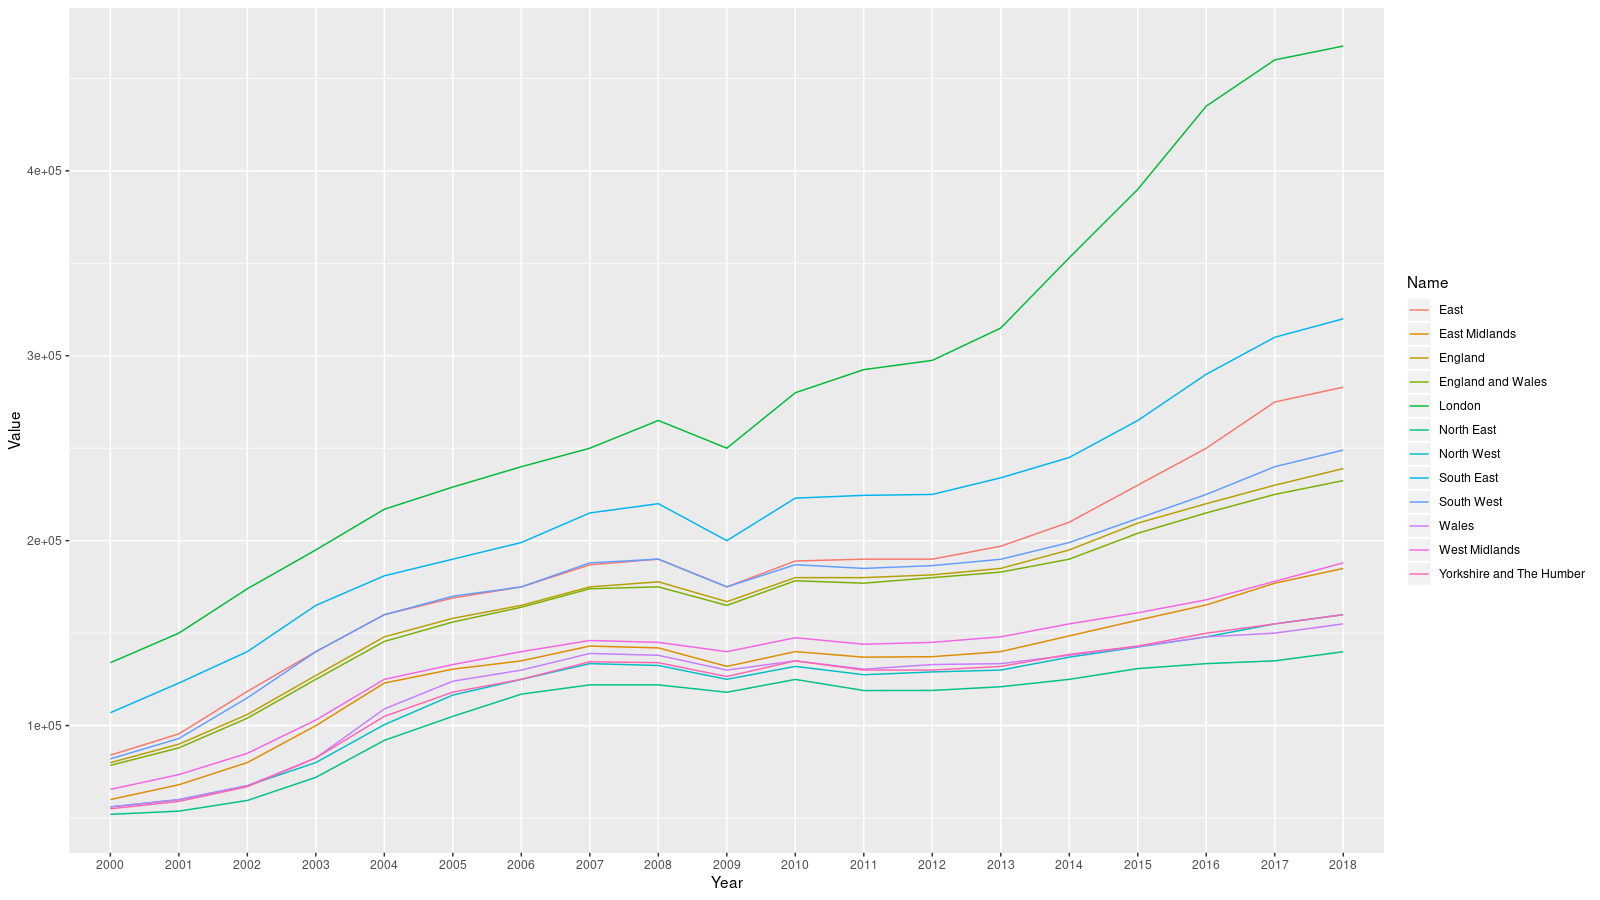
\includegraphics[width=8.5cm]{Q1Geom_line}}
  %  \vspace{2.0cm}
    \centerline{Question 1: Result 1}\medskip
  \end{minipage}
\end{figure}

This line graph illustrates the median house prices in nine regions of England and Wales from 2000 to 2018. 
England and Wales are also treated as regions and also England and Wales combined. Therefore, there 12 lines in the graph that represent 12 regions individually. 

The overall tendency of change for all regions is quite similar. Although fluctuated for a few years around 2009, 
the median house price in 12 regions was all increased from 2000 to 2018. Starting from 2000, the median house price in most region rose steadily until 2014. From 2004 to 2008, for all the regions, the increase in
median house price was slowing down comparing to the increase from 2000 to 2004. For the first time from 2000, the median house price in all regions suddenly dropped to the level of two years before. Then in 2009, the median house price in all regions bounced back to the highest level from 2000. From 2010 onward, the median house price was almost fixed for 3 years. Starting from 2013, the median hose price started increasing steadily for most regions but London. Median house price in London experienced a sharp increase from 2013 to 2017, 
as a result, the median house price increased by 1/3 compared to the data in 2013. From 2017 onward, 
the increase was slowing down again.

This line graph as an example is expressive and efficient when representing time-series data or the changing of quantitative during a continuous period of time. But sometimes, it is not appropriate for conducting the comparison. Therefore, the second graph was obtained using the same median house price data.

\begin{figure}[H]
  \begin{minipage}[b]{1.0\linewidth}
    \centering
    \centerline{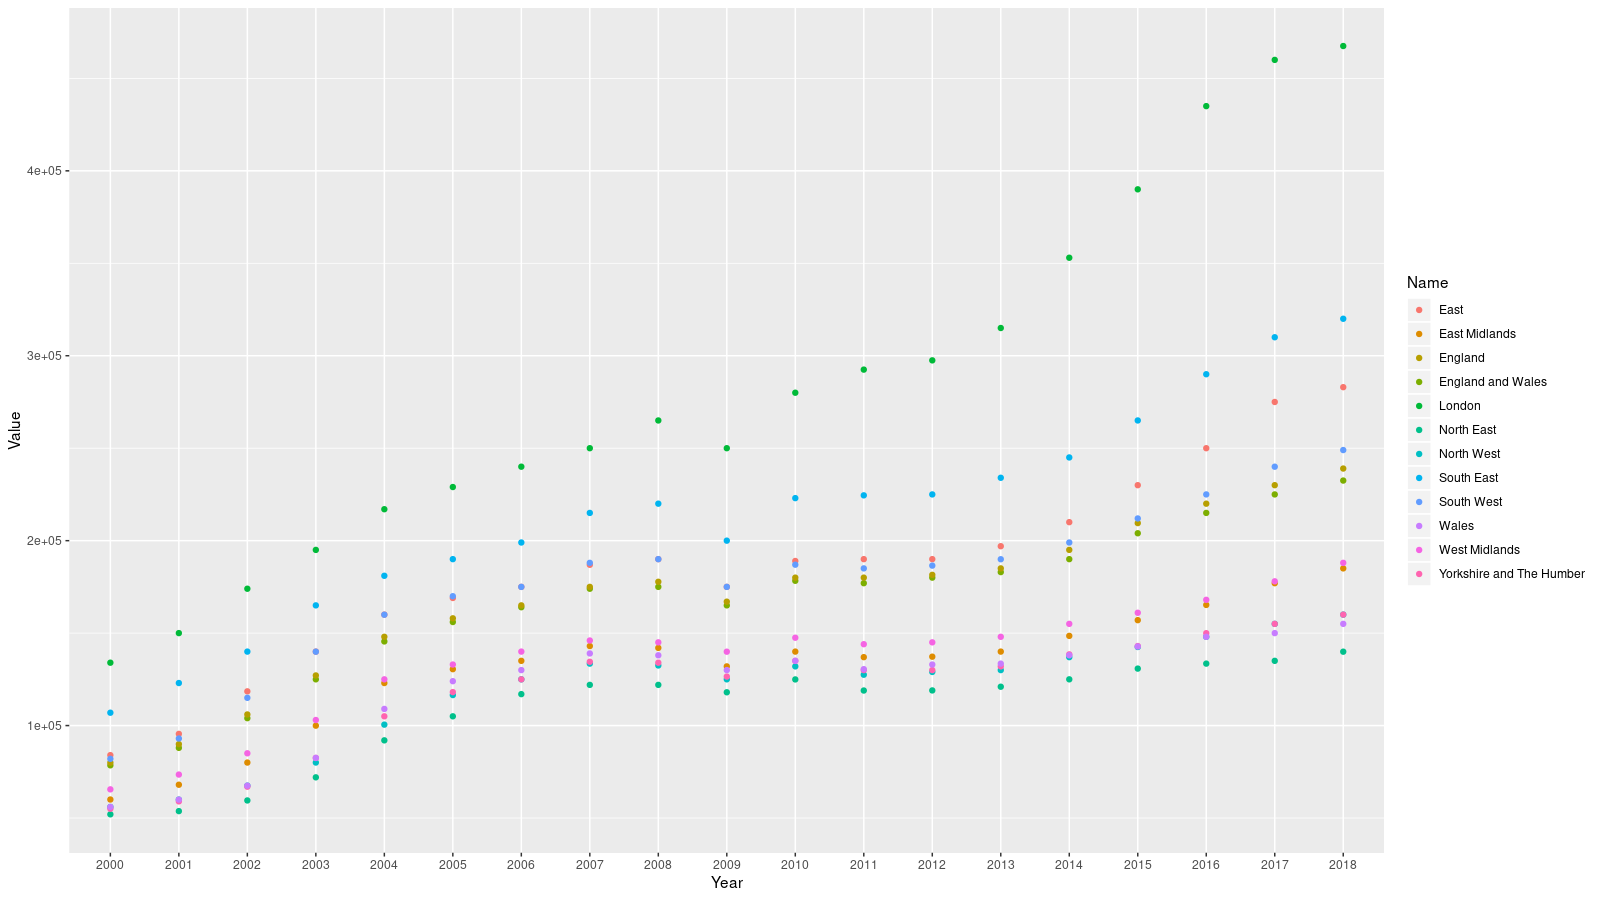
\includegraphics[width=8.5cm]{Q1Geom_point}}
  %  \vspace{2.0cm}
    \centerline{Question 1: Result 2}\medskip
  \end{minipage}
\end{figure}

This dot plot shows the same information as the line graph before but using a different representation. 
By using dot to exhibit the median house price for each region, the comparison of price between different 
regions are quite obvious compared to the line graph due to the overlap of lines can be observed in the line graph 
which caused diffculty to do the comparison.

Based on the dot plot, it is self-evident that the north east region has houses with the lowest median price 
from 2000 to 2018 while London has the most expensive houses.

\begin{figure}[H]
  \begin{minipage}[b]{1.0\linewidth}
    \centering
    \centerline{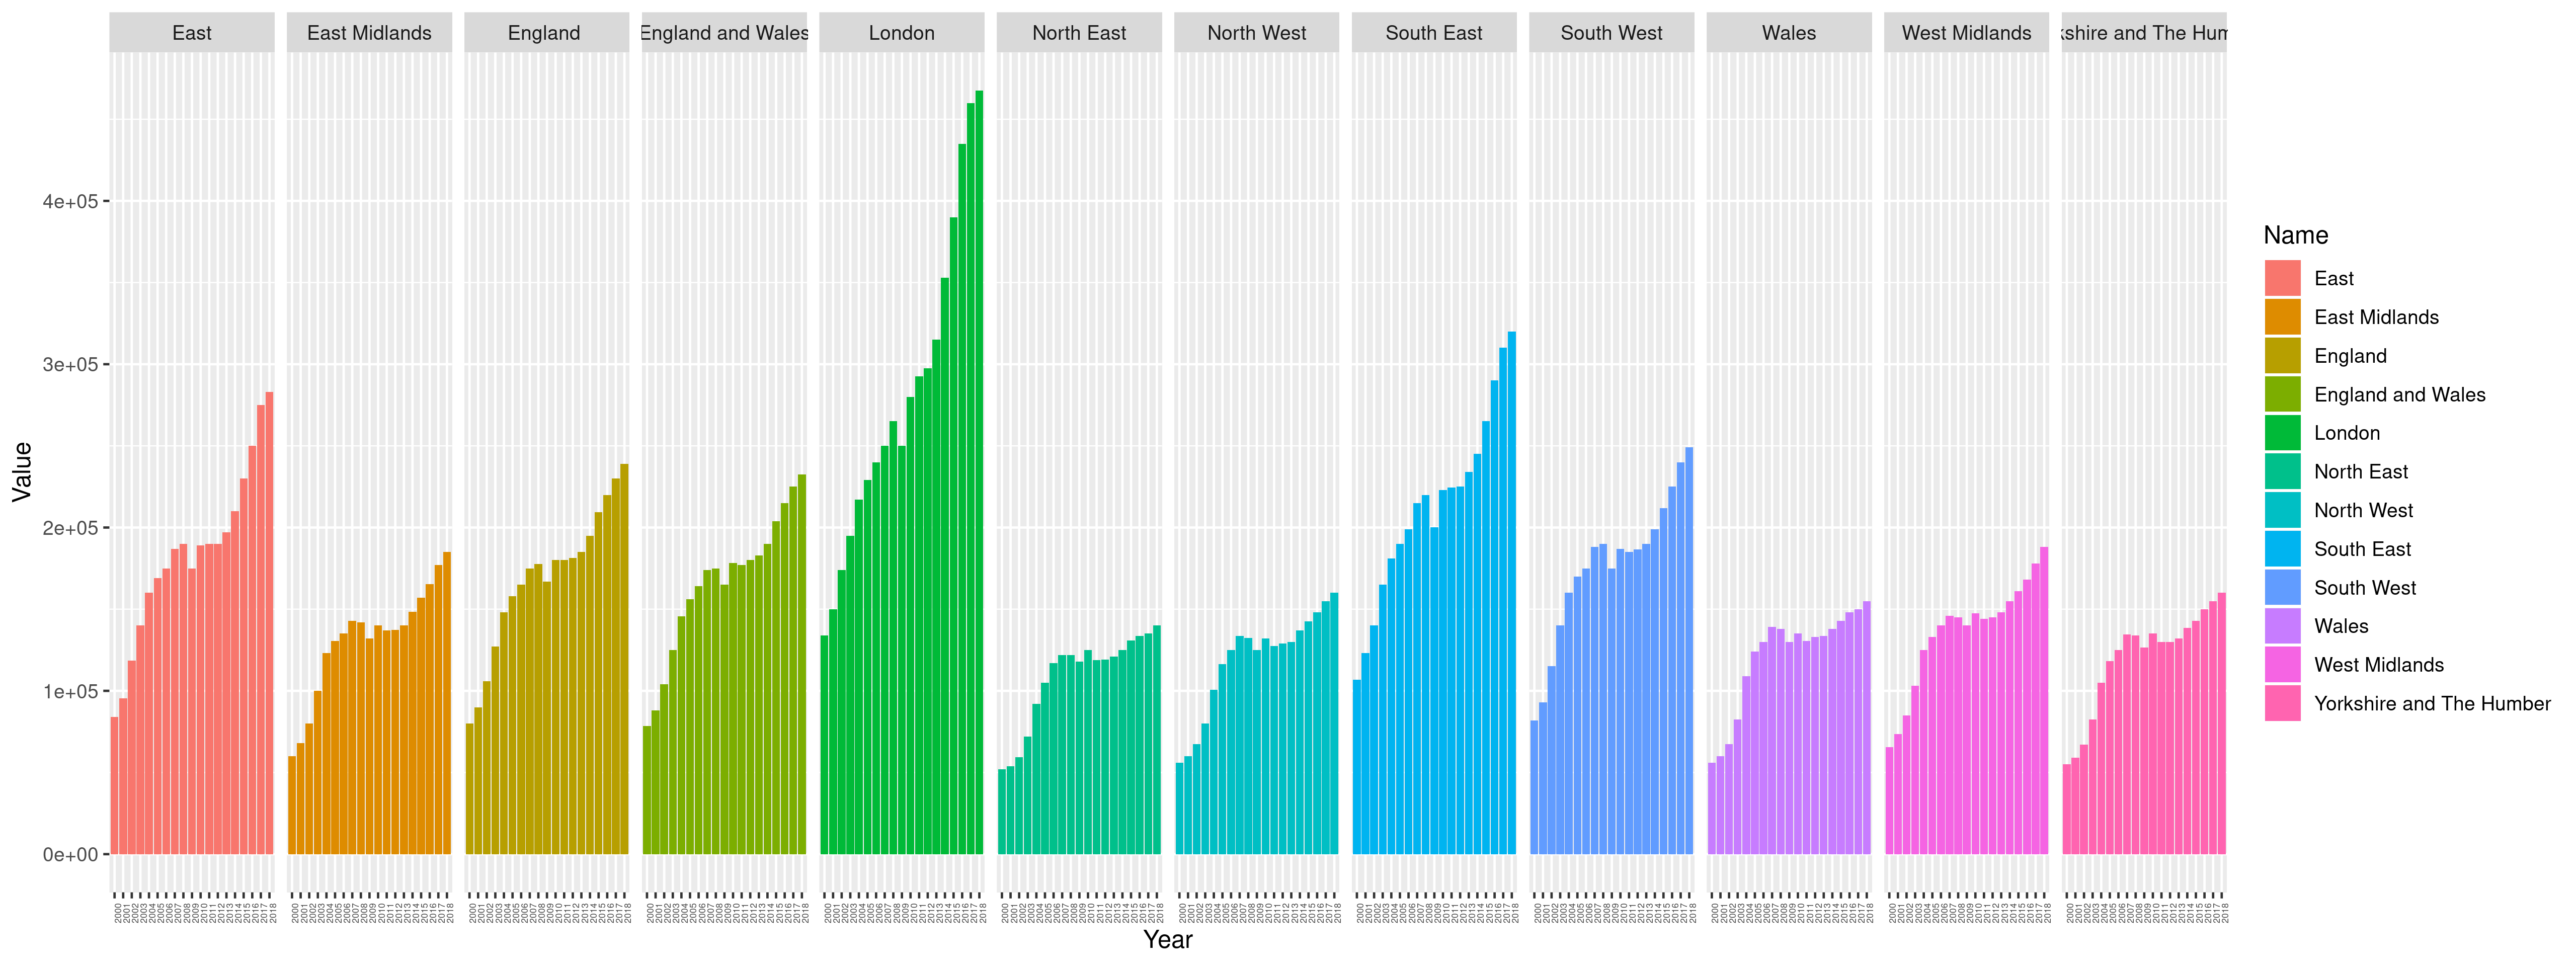
\includegraphics[width=8.5cm]{Q1Geom_gridbar}}
  %  \vspace{2.0cm}
    \centerline{Question 1: Result 3}\medskip
  \end{minipage}
\end{figure}

The last graph for the house price visualisation part is a bar chart which was gained using the same median house price data. This bar chart illustrates the median house price of 12 regions from 2000 to 2018 
grouped by region. This graph has an advantage over the line graph and dot plot when studying the changes of median house price of individual regions as it combines the benefit of those two while makes data related to individual region evident.

\subsubsection{Visual Encodings}
Based on Bertin's semiology graphics \cite{BertinJacques}, the following characteristics of visual encoding variable are taken into consideration during the visualisation process. 

\begin{itemize}
  \item Selective:
        whether the changes of a variable can make the variable distinctive from the group
  \item Associative:
        whether the changes of a variable can be interperted together as a group
  \item Quantitative: 
        whether the numerical measures can be identified from the changes of a variable
  \item Length:
        how many recognisable changes can be indentified in a variable
\end{itemize}

Combined with the characteristics listed above, there are two principles of choosing visual encodings that also need to be enforced. The principle of consistency refers to the properties of the visual variable should match 
the properties of data and the principle of importance ordering refers to encoding the most essential information 
in the most practical manner.

In terms of the line graph for this question, position and hue are selected for the graph. As a visual variable, 
position possesses characteristics like selective, associative and quantitative. Moreover, as for the length characteristics, theoretically, it can be infinite. While hue is selective and associative. As for length, 
the limitation of length when using hue is hardly applied to this dataset. But without hue, the graph is not effective nor expressive(See Appendix 1). By combining position and hue together, the line graph was drawn. 

Judging from the design criteria, the line graph satisfies expressiveness, and partial effectiveness because the dot plot is more effective when compare house prices for all regions by year. In addition, by enforcing 
the principle of importance ordering the dot plot was obtained to address this issue.

As for the bar chart, position and hue are combined to achieve expressiveness and effectiveness. It turns out 
that the bar chart is more effective than the line graph and dot plot when studying the house price of an individual region.




\subsection{Affordability Visualisation}
Stated in the initial question section, the second question is intended to examine how the affordability ratio changed from 2000 to 2018 
and to further probe which region has the most affordable house. Due to the similar nature of the question, 
similar approaches for house price visualisation can be applied here. As data processing operations described above. 
The first graph can be obtained.

\begin{figure}[H]
  \begin{minipage}[b]{1.0\linewidth}
    \centering
    \centerline{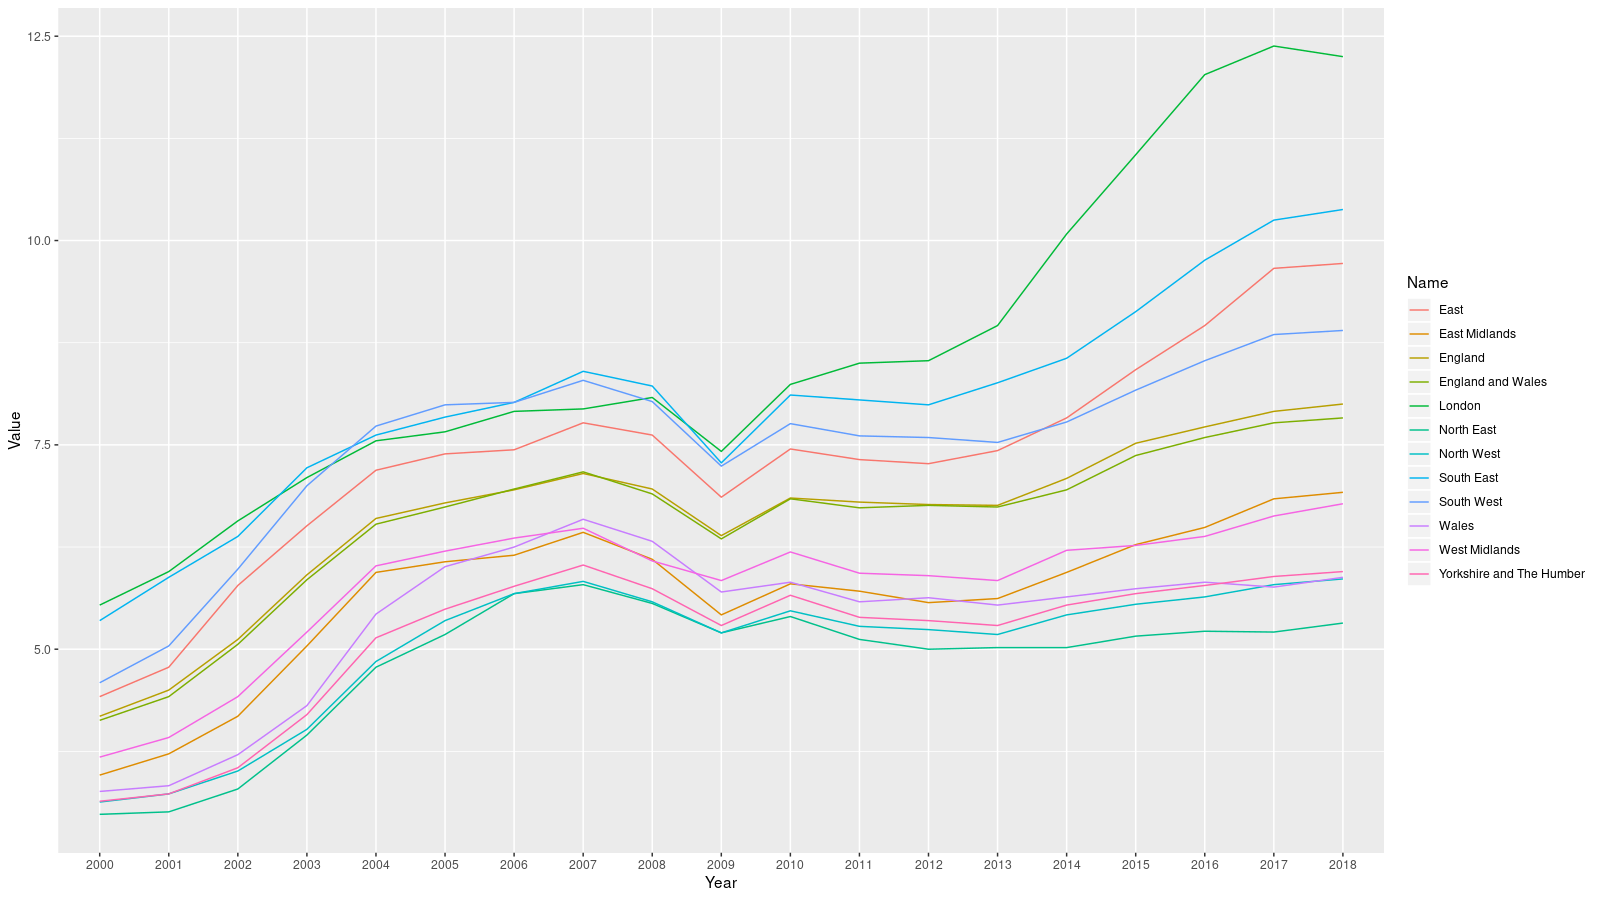
\includegraphics[width=8.5cm]{Q2Geom_line}}
  %  \vspace{2.0cm}
    \centerline{Question 2: Result 1}\medskip
  \end{minipage}
\end{figure}

This line graph illustrates the affordability ratio in nine regions of England and Wales from 2000 to 2018. 
England and Wales are also treated as regions and also England and Wales combined. Therefore, there 12 lines in the graph that represent 12 regions individually. As the name suggested, the affordability ratio is the ratio of median house price to the median workplace-based earnings. Therefore, the lower the ratio, the more 
affordable the houses are in a region.

The general trend of change for all regions is identical. Although flucuated for a few years around 2009, 
the affordability ratio in 12 regions was all increased from 2000 to 2018. Starting from 2000, the affordability ratio in most regions rose steadily until 2001 and then continued to increase with a faster velocity until 2004. 
From 2004 to 2008, for all the regions, the increase of affordability ratio was almost static for most of the regions compared to the increase from 2000 to 2004. For the first time from 2000, the affordability ratio in all regions suddenly dropped to the level of four years before. Then in 2010, the affordability ratio in all regions bounced back, and from 2010 onward, the affordability ratio was almost fixed for 4 years. Starting in 2013, 
the affordability ratio started increasing steadily for most regions except London. The affordability ratio in London started growing from 2010 and experienced a sharp upward that last four year and it still increasing in 2018, 
as the result, the affordability ratio increased by more than 1/3 compared to the data in 2013. Starting from 2013, 
in most region, the affordability ratio started going upwards steadily until 2018.

This line graph as an example is expressive and efficient when representing time-series data or the changing of quantitative during a continuous period of time. But sometimes, it is not appropriate for conducting the comparison. Therefore, the second graph was generated using the same affordability ratio data.

\begin{figure}[H]
  \begin{minipage}[b]{1.0\linewidth}
    \centering
    \centerline{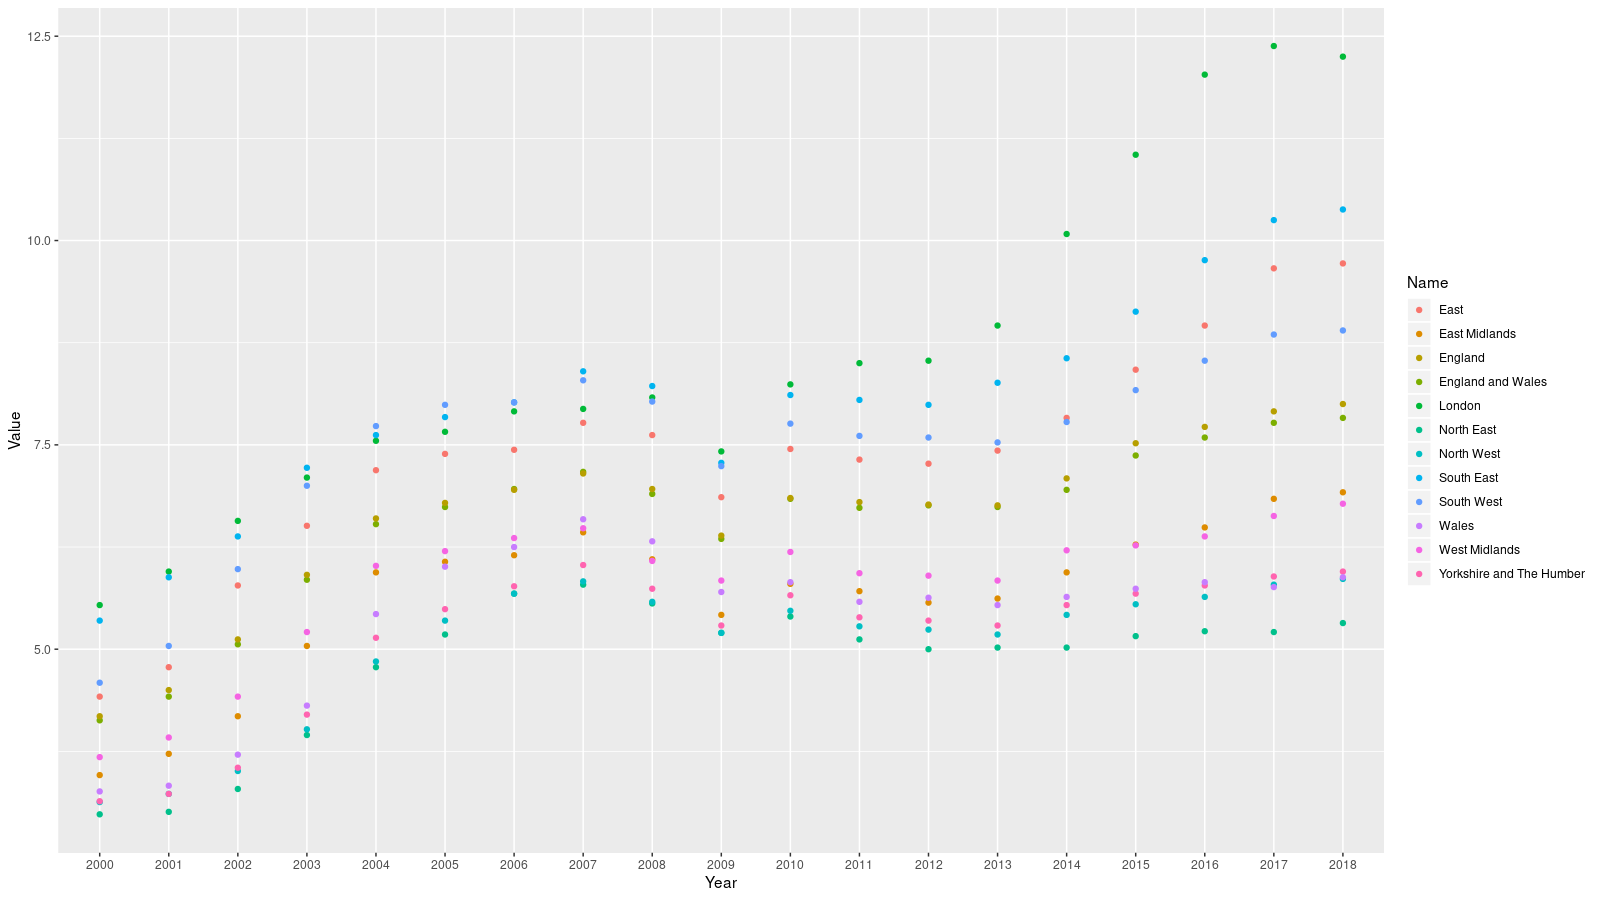
\includegraphics[width=8.5cm]{Q2Geom_point}}
  %  \vspace{2.0cm}
    \centerline{Question 2: Result 2}\medskip
  \end{minipage}
\end{figure}

This dot plot shows the same information as the line graph before but using a different representation. 
By using dot to exhibit the affordability ratio for each region, the comparison of the ratio between different 
regions are quite obvious compared to the line graph due to the overlap of the line can be observed in the line graph 
which caused diffculty to do the comparison.

Based on the dot plot, it is self-evident that the north east region has the most affordable houses from 2000 
to 2018. As the for least affordable houses, the results are interesting to compare to the house price. 
As demostrated in house price visualisation part, Houses in London always have the highest price from 2000 to 2018.
But the affordability ratio date suggests that from 2000 to lat 2002, the affordability ratio in London was the lowest across the regions but later on the affordability ratio of south-west and south-east surpassed the value of London. 
London did not possess the highest value of affordability ratio until late 2018, maintained its statue until 2018.


\begin{figure}[H]
  \begin{minipage}[b]{1.0\linewidth}
    \centering
    \centerline{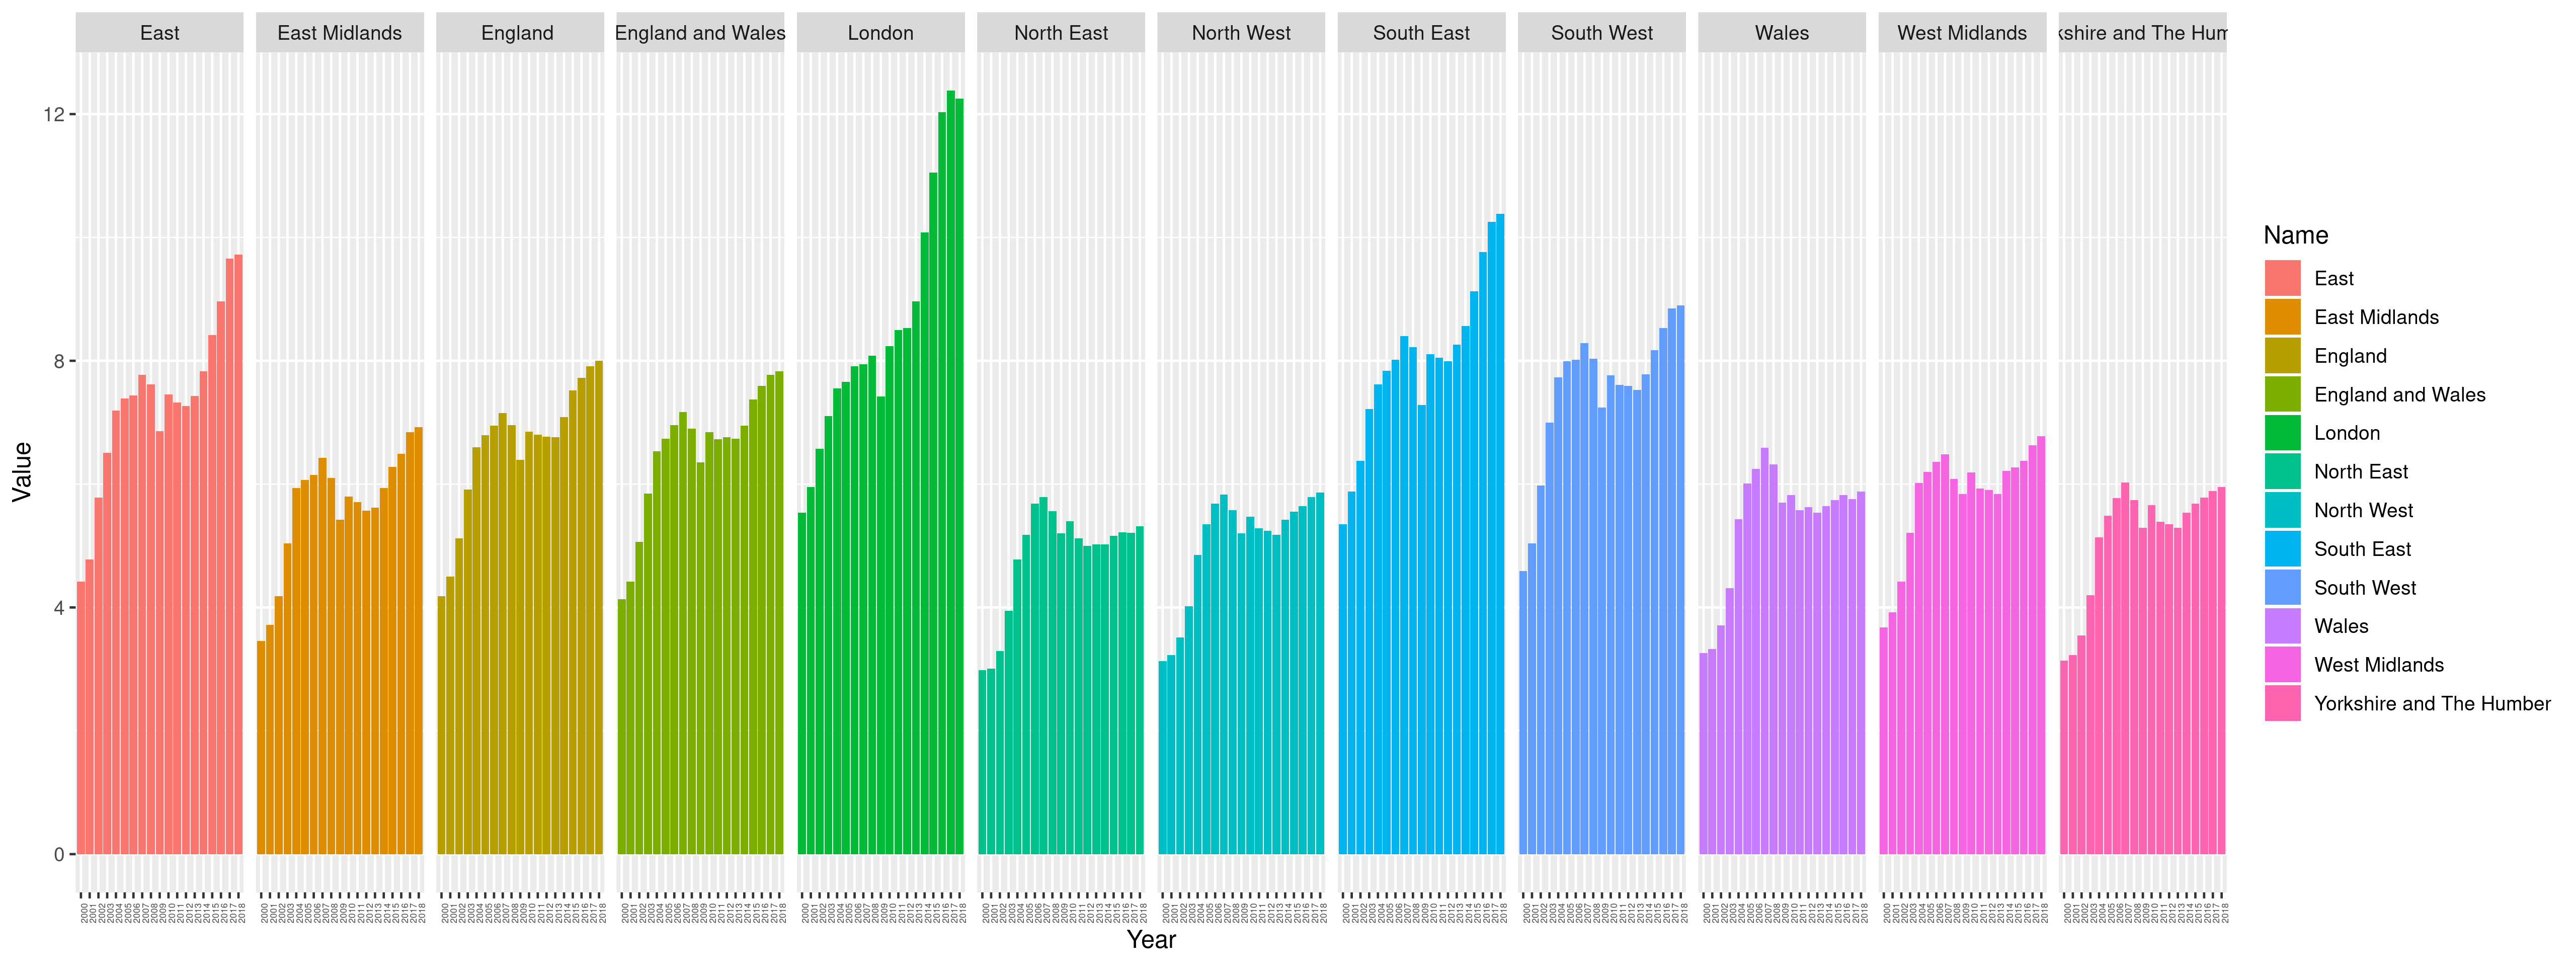
\includegraphics[width=8.5cm]{Q2Geom_gridbar}}
  %  \vspace{2.0cm}
    \centerline{Question 2: Result 3}\medskip
  \end{minipage}
\end{figure}

The last graph for the affordability ratio visualisation part is a bar chart which was gained using the same affordability ratio data. This bar chart illustrates the affordability ratio of 12 regions from 2000 to 2018 
grouped by region. This graph has an advantage over the line graph and dot plot when studying the changes of affordability ratio of individual regions as it combines the benefit of those two while makes data related to individual region evident.

\subsubsection{Visual Encodings}
Due to the nature of the affordability visualisation, similar approaches used to visualise the house price can be employed.

In terms of the line graph for this question, position and hue are selected for the graph. The fitnesses of using position and hue discussed for visual encodings of the house price question can also be applied here. 
Moreover, according to Mackinlay's effectiveness ranking(See Appendix 2)\cite{MackinlayJock1986Atdo}, 
position as a visual variable is the best fit for quantitative, ordinal and nominal data. For nominal data, 
position and hue are both competent encodings. Therefore, by combining position and hue, a higher level of expressiveness and effectiveness for encoding nominal can be achieved. The line graph as stated employed all the techniques discussed above. 

Judging from the design criteria, the line graph satisfies expressiveness, and partial effectiveness because the dot plot is more effective when compare affordability ratio for all regions by year. In addition, by enforcing 
the principle of importance ordering the dot plot was obtained to address this issue.

As for the bar chart, position and hue are combined to achieve expressiveness and effectiveness. It turns out 
that the bar chart is more effective than the line graph and dot plot when studying the house price of an individual region.


\subsection{Impact of Economy Crisis}
The last initial question is to audit the impact the economic crisis has on house price and affordability
in 12 regions. In this case, the date ned to be processed further. As the economic crisis happened in 2018, 
the comparison of the data in 2008 and 2009 would depict the immediate impact of the economic crisis. By taking in consideration of median house price, annual earnings and affordability ratio, the bar chart can be gained.

\begin{figure}[H]
  \begin{minipage}[b]{1.0\linewidth}
    \centering
    \centerline{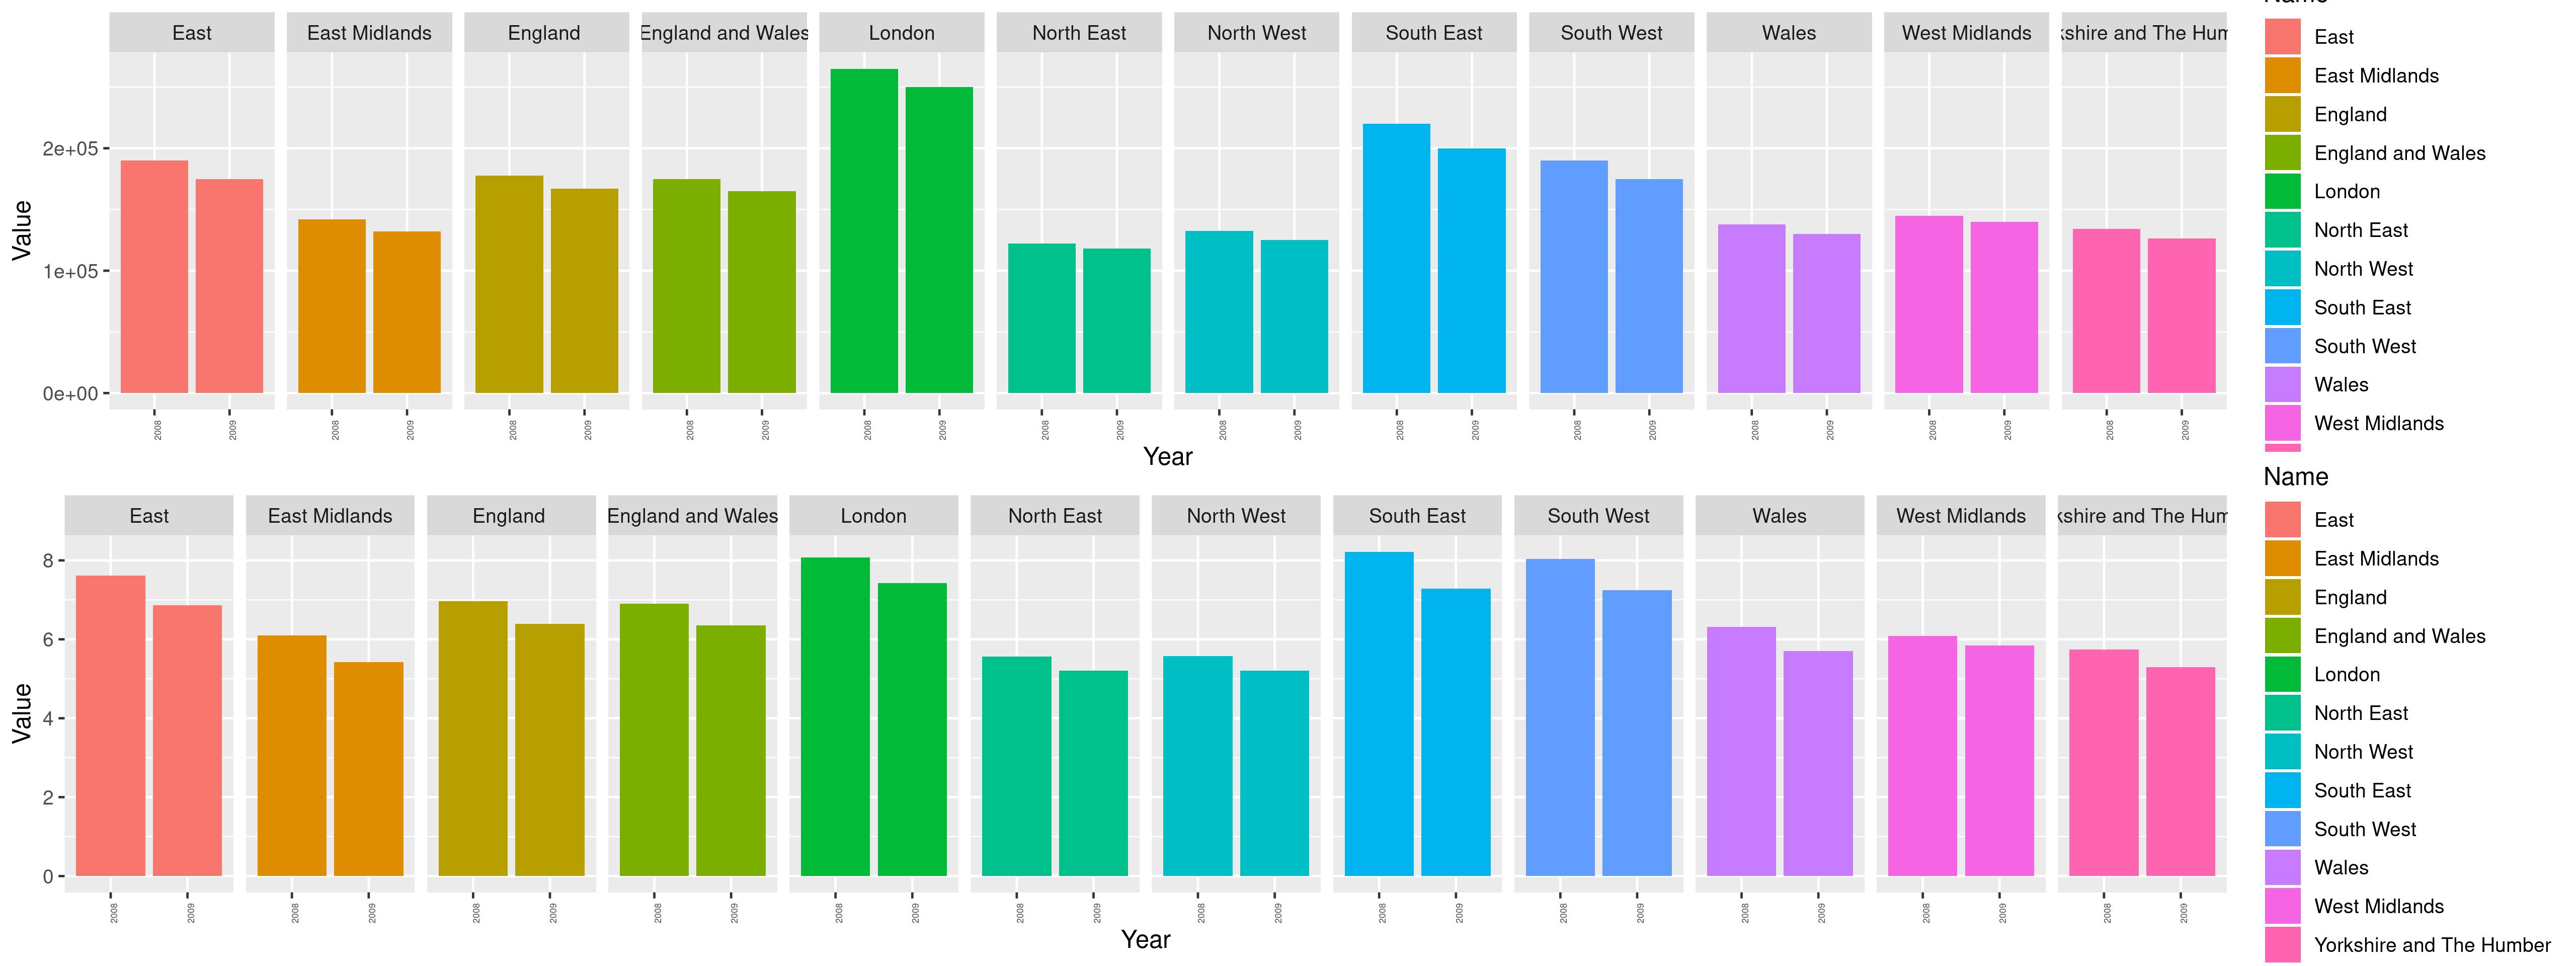
\includegraphics[width=8.5cm]{Q3Geom_gridbar}}
  %  \vspace{2.0cm}
    \centerline{Question 3: Result}\medskip
  \end{minipage}
\end{figure}

This bar chart combines the data of median house price, median annual gross workplace-based earnings and affordability ratio from 2008 to 2009. This chart is intended to show the immediate impact of the economic crisis in 2008. As the graph shows, the first row indicates the annual earning data, the second row represents the median house price data and the last row suggests affordability ratio. 

As the graph demonstrated, the economic crisis did not seem to have serve impact on annual earnings as the annual earnings did not experience any regression in any region. In contrast, the impact of the economic crisis on house price was obvious, the house price decreased in all 12 regions. By combining these data, the annual earnings increased slightly while the house price decreased, as a result, the affordability ratio decreased. The diminish of affordability ratio suggested that the houses in all 12 regions became more affordable as an impact of economic crisis. 

\subsubsection{Visual Encodings}
According to Bertin's semiology of graphics and Mackinlay's effectiveness ranking, although, line graph and 
dot plot fulfils the principle of consistency and importance ordering, they are not fit for studying this question 
as they cannot achieve effectiveness and expressiveness in term of this question. Hence, the bar chart was 
chosen for this question and position and hue are still used.

This question is to find out the impact of the economic crisis by comparing data in 2008 and 2009. Therefore, by representing data in two years using the bar chart and grouped by region, the answer can be self-evident. 
By visualising data of median house price, annual earnings and affordability ratio seperately and put 
together in the bar chart, effectiveness and expressiveness are achieved at an appropriate level to answer
this question.


\subsection{Correlation Coefficients of House Price}
As the graphs are shown in house price visualisation and affordability ratio visualisation section, the general tendency in those regions were quite akin. So that result leads to another question, whether the house prices in those regions were related and if they were related to how closely they are related to each other.

In search of this question, further data transformation is needed. The column in the dataset which identity time can be omitted. Furthermore, each region was put in a separate column with all of the data related to the region sorted by time. The correlation coefficient is numerical measure the can reveal how different entities are related to each other. After this transformation, the correlation coefficients can be calculated. Hence, 
the heat map contains correlation coefficients can be obtained.

\begin{figure}[H]
  \begin{minipage}[b]{1.0\linewidth}
    \centering
    \centerline{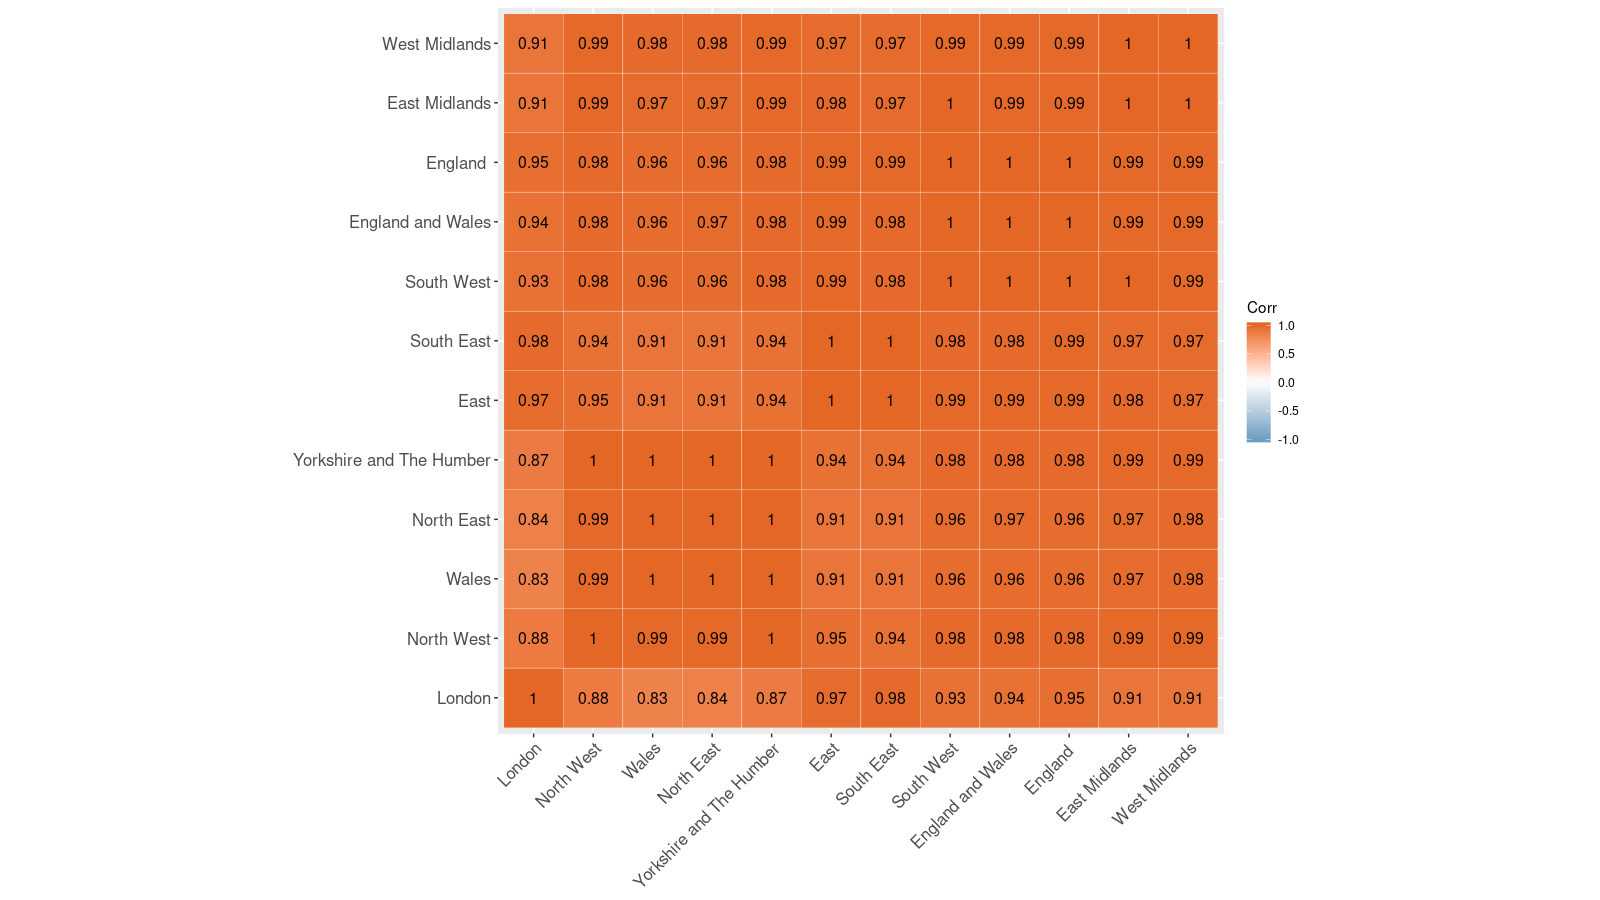
\includegraphics[width=8.5cm]{corHeatMap}}
  %  \vspace{2.0cm}
    \centerline{Correlation Coefficients: Result}\medskip
  \end{minipage}
\end{figure}

As the heat map shows, the correlation coefficients scale from 1 to -1. The closer the correlation coefficients 
to 1 the more they are related and vice versa.

As the data suggests, house prices in most regions are highly correlated as most of the correlation coefficients are above 0.9. Despite correlation coefficients between some regions are below 0.9, they still can be 
considered closely related as they all surpassed 0.8.

\subsubsection{Visual Encodings}
For the correlation coefficients, they are calculated in pairs and stored in tabular form, which makes the heatmap an appropriate visualisation representation. Heatmap visualises changes in colouring, which is an advantage to visualise data in tabular form while revealing variance by cross-examining between multivariate data.

Due to heatmap communicating values by using colours, sometimes it hard to distinguish accurately between values which lead to expressiveness and effectiveness issues. To addressing this, accurate data was put on top of the cell to achieve expressiveness and effectiveness at an appropriate level.



\section{Evaluation}
The general process of this research is based on the procedures proposed by Fry\cite{Fry}. According to Fry\cite{Fry}, 
the seven stages of visualisation are acquire, parse, filter, mine, represent, refine and interact.
Since there is no interaction part for this project, the interacting process is omitted. Furthermore, 
these stages can be generalised into two groups, data processing and information visualisation. Acquire, parse, 
filter, mine are included in data processing and the rest are included in the information visualisation process. 

There are challenges after the information visualisation process when conducting the evaluation process.
For all the questions proposed above, conclusion validity is the main concern as the validity of the final result depends on it. Specifically for the third initial question, internal validity is an essential factor to consider as the nature of the question is to find out the relationship between the impact of economic crisis and house price. Finally, the construct validity and external validity are solid for this project due to 
the ideas this study is based on are obvious and the results are distinctive.

By following stages mentioned above, this project started with data processing and then to visualisation. The goal 
of this project is to explore the question proposed earlier and finally, the goal is achieved by answering proposed 
question using information visualisation techniques.





% To start a new column (but not a new page) and help balance the last-page
% column length use \vfill\pagebreak.
% -------------------------------------------------------------------------
%\vfill
%\pagebreak


\vfill\pagebreak
\printbibliography

\vfill\pagebreak
\section*{Appendix}
\subsection{Appendix 1}
\begin{figure}[H]
  \begin{minipage}[b]{1.0\linewidth}
    \centering
    \centerline{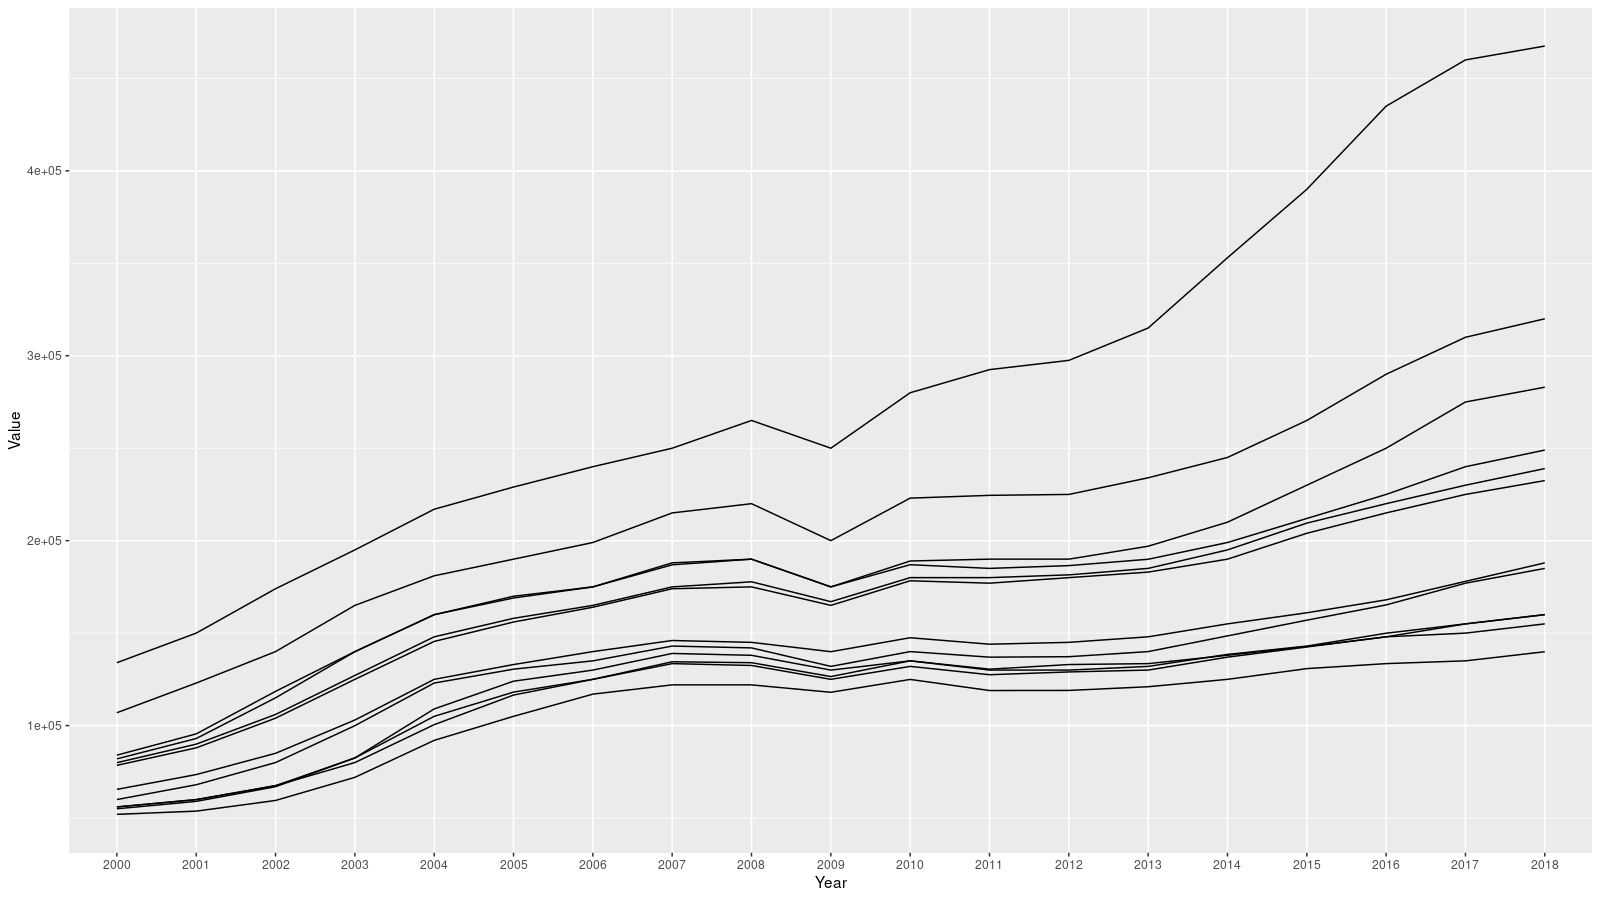
\includegraphics[width=8.5cm]{Q1Geom_line_no_colour}}
  %  \vspace{2.0cm}
    \centerline{Q1 Line Graph No Colour}\medskip
  \end{minipage}
\end{figure}

\begin{figure}[H]
  \begin{minipage}[b]{1.0\linewidth}
    \centering
    \centerline{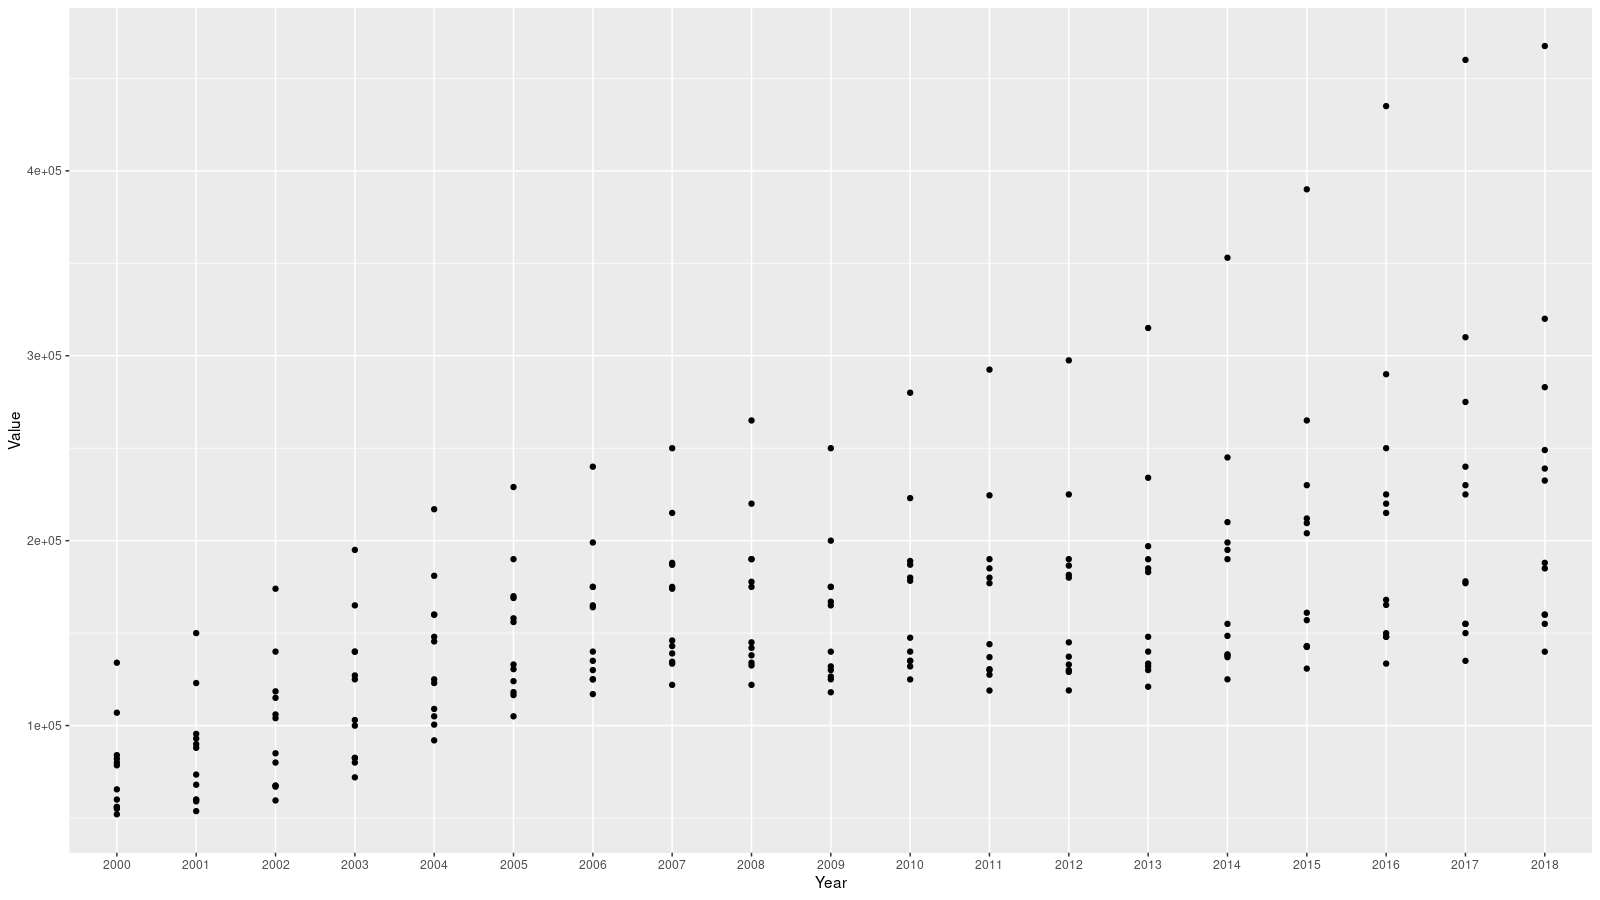
\includegraphics[width=8.5cm]{Q1Geom_point_no_colour}}
  %  \vspace{2.0cm}
    \centerline{Q1 Dot Plot No Colour}\medskip
  \end{minipage}
\end{figure}

\begin{figure}[H]
  \begin{minipage}[b]{1.0\linewidth}
    \centering
    \centerline{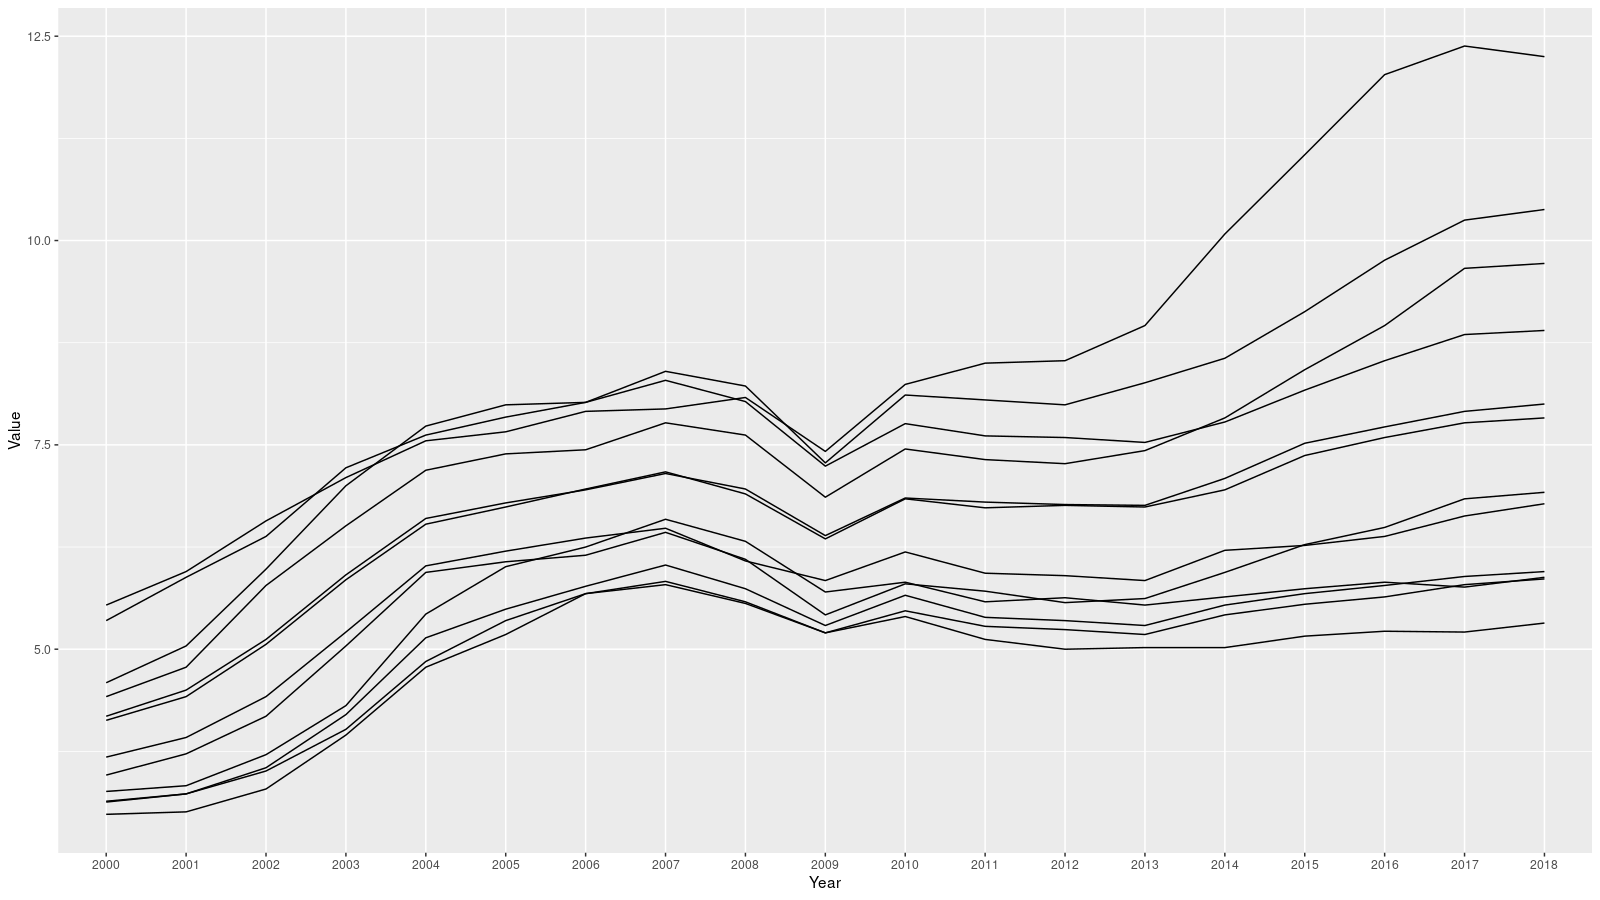
\includegraphics[width=8.5cm]{Q2Geom_line_no_colour}}
  %  \vspace{2.0cm}
    \centerline{Q2 Line Graph No Colour}\medskip
  \end{minipage}
\end{figure}

\begin{figure}[H]
  \begin{minipage}[b]{1.0\linewidth}
    \centering
    \centerline{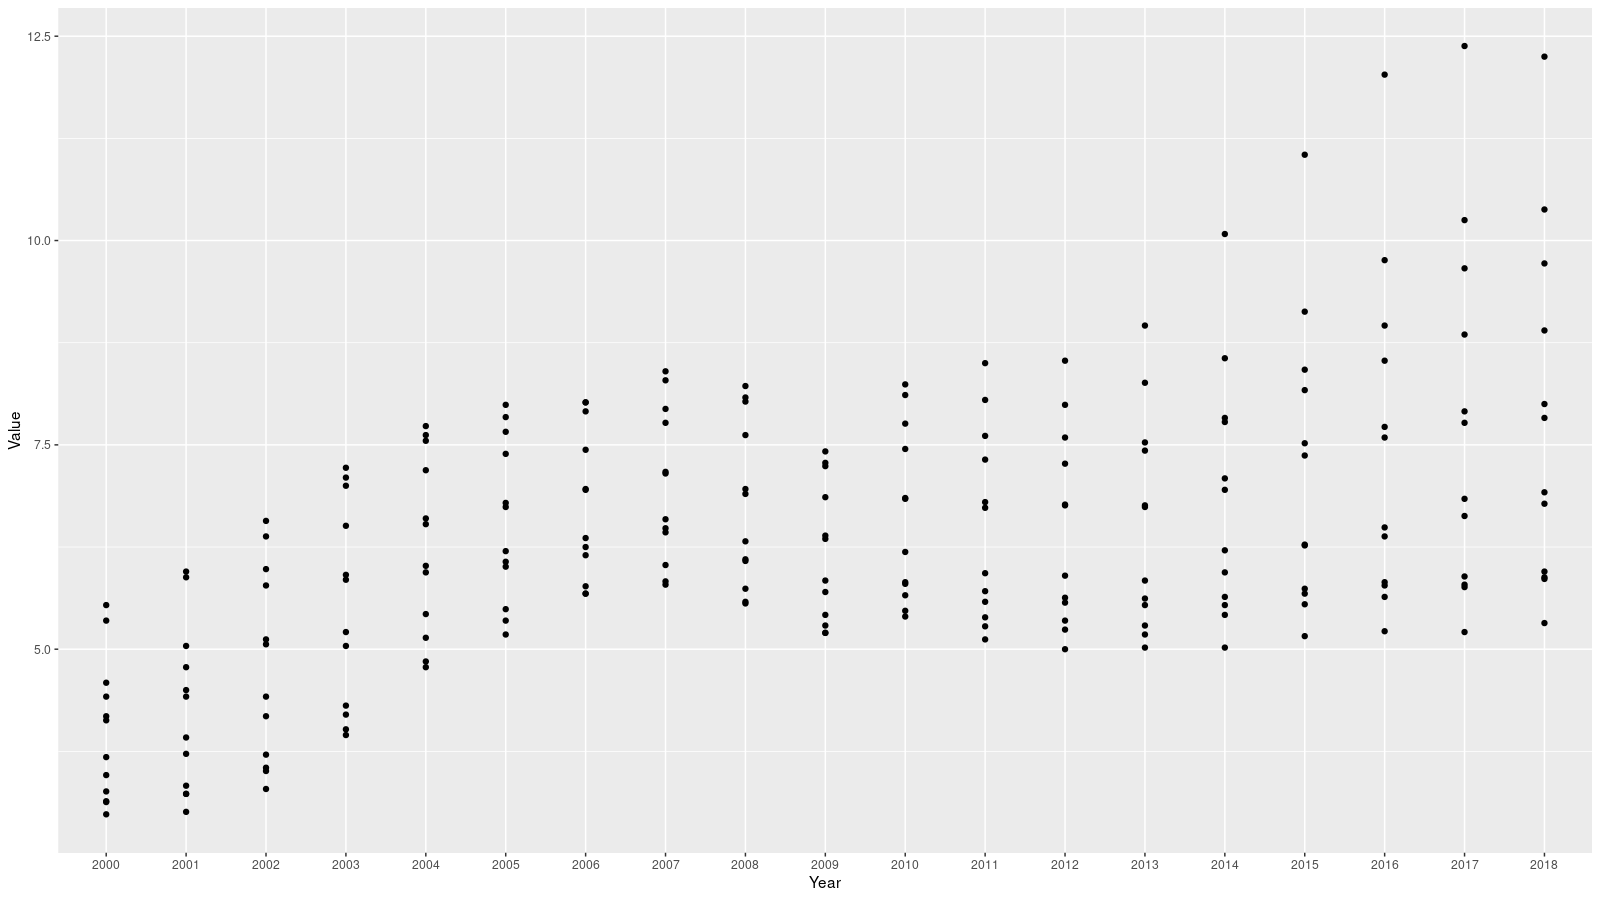
\includegraphics[width=8.5cm]{Q2Geom_point_no_colour}}
  %  \vspace{2.0cm}
    \centerline{Q2 Dot Plot No Colour}\medskip
  \end{minipage}
\end{figure}

\subsection{Appendix 2}
\begin{figure}[H]
  \begin{minipage}[b]{1.0\linewidth}
    \centering
    \centerline{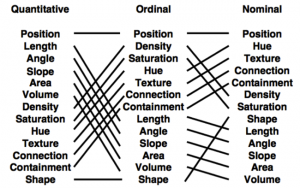
\includegraphics[width=8.5cm]{mackinlayRankings}}
  %  \vspace{2.0cm}
    \centerline{Mackinlay's Effectiveness Ranking}\medskip
  \end{minipage}
\end{figure}



\end{document}
